\newcommand{\figurescaling}{0.7}
\documentclass[a4paper,oneside,parskip=half]{scrartcl}

\usepackage{graphicx}
\usepackage{natbib}
\usepackage[utf8]{inputenc}
\usepackage{tabularx}
\usepackage{hyperref}
\usepackage{color}
\usepackage[usenames,dvipsnames,svgnames,table]{xcolor}
\usepackage{longtable}
\usepackage{slashbox}
\usepackage{multirow}
\usepackage{minibox}
\usepackage{placeins }
\usepackage{booktabs}
\usepackage[UKenglish]{babel}
\usepackage[T1]{fontenc}
\usepackage{lmodern}
\usepackage{pifont}
\usepackage{paralist}
\usepackage{listings}
\usepackage{enumitem}
\usepackage{multicol}
\usepackage[utf8]{inputenc}
\usepackage{authblk}

\title{Machine Learning WS2013}
\subtitle{Assignment 3 \\[0.8cm] {\rmfamily\normalfont\Large}}

\author[1]{Dino Rossegger}
\author[2]{Navid Rekabsaz}
\author[3]{Soroosh Mortezapoor}
\affil[1]{e0926471@student.tuwien.ac.at}
\affil[2]{e1129057@student.tuwien.ac.at}
\affil[3]{soroosh.mortezapoor@student.tuwien.ac.at}

\lstset{language=java,basicstyle=\ttfamily\footnotesize}

\begin{document}

\maketitle
\begin{abstract}
\end{abstract}

\section{Task}
The task was to analyse the differences in different feature selection techniques, i.e. analyse the difference in the selected features of the techniques. Therefore a java program had to be developed using the weka library to run the feature selection techniques on different datasets supplied by the lectors.

Furthermore a comparison of the results of k-nn using the top $n$ features of each feature selection technique and using mutual features was to be done. This was also implemented in the program using weka.

\section{Program Usage}
The java program uses ant to allow easy building and running of the program. In the build file the two properties \lstinline$weka.dir$ and \lstinline$lib.dir$ (containing apache commons cli) need to be changed.
Afterwards the program can be compiled using \lstinline$ant compile$, it is suggested to create a jar file using \lstinline$ant jar$.

The program accepts a number of arguments, in Listing~\ref{list:helpoutput} the help output can be seen. The only obligatory flag is \lstinline$-d <directory>$, specifying the directory from which the instances should be read. The rest of the arguments are optional, the help output in Listing~\ref{list:helpoutput} should be enough aid in understanding the usage of the program.
\begin{lstlisting}[caption=help output of the program, label=list:helpoutput]
 -c               compare results and find mutual features of result files
                   inside a directory
 -d <directory>   directory with instancefiles in csv or arff format
 -f <technique>   use specified feature selection technique
 -h               display this usage information
 -l               list all available feature selection techniques
 -n <n>           use top <n> attributes, default: 10
 -t <f>           consider attributes appearing in f per cent of the
                   result sets, default: 0.5

\end{lstlisting}
First the specified techniques (or all implemented techniques if \lstinline$-f$ is not set) are applied to the datasets, then the selected attributes are compared. At last a classifier is run using the features obtained from the feature selection methods. The precision, recall and f1-scores of the runs are printed on standard output.

\section{Technique Comparison}
In this section, we describe applied techniques and compare their selected attributed in order to understand how (dis)similar different algorithms are.

Applied techniques are described in Table\ref{table:techniques}. As it is shown eight supervised as well as two unsupervised algorithms are developed and used.

Since both unsupervised methods (PCI and LSA) reduce the input data to another matrix, the final attributes in reduced
matrix are not comparable with input data. In the case of applying Ranker search method on any of unsupervised evaluators, the ranked attributes will be a sequence from one to the number of attributes. Therefore, we decided to focus more on behavior of supervised methods.

We apply program's algorithm comparison ($-c$ parameter) on the result of eight supervised algorithms. Using provided data, we understand the number of mutual attributes between each pair of algorithms. in order to apply clustering on the methods, distance matrix is created. In order to form the matrix, the number of mutual attributes for each pair are subtracted from $50$. The distance matrix of $GTZAN$ dataset is shown in Table\ref{table:distancematrix}.

In the next step, by using R the methods are clustered based on Hierarchal Clustering algorithm. The clustering results of four datasets are shown in Figure\ref{fig:clustering}.

Based on the diagrams, following results can be concluded:
\begin{itemize}
\item ChiSquaredAttribute and InfoGain tend to have very similar results.
\item Besides ChiSquaredAttribute and InfoGain, SymmetricalUncertAttribute is the most similar one to them.
\item ConsistencySubset has always the most different results in comparison to the others.
\item CfsSubset and ReliefFAttribute seems to be related in some cases.
\end{itemize}

\begin{table}[p]
\begin{center}
\begin{tabular}{|c|c|c|c|}
\hline Attribute Evaluator & Search Method & Supervised/Unsupervised & Parameter Name \\
\hline CfsSubset & GreedyStepwise & Supervised & cfs-greedy\\
\hline ChiSquaredAttribute & Ranker & Supervised & chis-ranker\\
\hline ConsistencySubset & BestFirst & Supervised & cons-bestfirst\\
\hline GainRatioAttribute & Ranker & Supervised & gainr-ranker\\
\hline InfoGain & Ranker & Supervised & ig-ranker\\
\hline OneRAttribute & Ranker & Supervised & oner-ranker\\
\hline ReliefFAttribute & Ranker & Supervised & rel-ranker\\
\hline SymmetricalUncertAttribute & Ranker & Supervised & sua-ranker\\
\hline PrincipalComponents & Ranker & Unsupervised & pca-ranker\\
\hline LatentSemanticAnalysis & Ranker & Unsupervised & lsa-ranker\\
\hline
\end{tabular}
\caption{Applied attribute selection techniques}
\label{table:techniques}
\end{center}
\end{table}


\begin{table}[p]
\begin{center}
\begin{tabular}{|c|p{1.3cm}|p{1.3cm}|p{1.3cm}|p{1.3cm}|p{1.3cm}|p{1.3cm}|p{1.3cm}|p{1.3cm}|}
\hline & cfs-greedy & chis-ranker & cons-bestfirst & gainr-ranker & ig-ranker & oner-ranker & rel-ranker & sua-ranker\\
\hline cfs-greedy & 0 & 41 & 46 & 44 & 40 & 39 & 28 & 40\\
\hline chis-ranker & 41 & 0 & 48 & 39 & 9 & 21 & 37 & 9\\
\hline cons-bestfirst & 46 & 48 & 0 & 50 & 48 & 49 & 47 & 49\\
\hline gainr-ranker & 44 & 39 & 50 & 0 & 37 & 34 & 41 & 34\\
\hline ig-ranker & 40 & 9 & 48 & 37 & 0 & 16 & 36 & 4\\
\hline oner-ranker & 39 & 21 & 49 & 34 & 16 & 0 & 37 & 16\\
\hline rel-ranker & 28 & 37 & 47 & 41 & 36 & 37 & 0 & 36\\
\hline sua-ranker & 40 & 9 & 49 & 34 & 4 & 16 & 36 & 0\\
\hline
\end{tabular}
\caption{Applied attribute selection techniques}
\label{table:distancematrix}
\end{center}
\end{table}


\begin{figure}[p]
\begin{center}
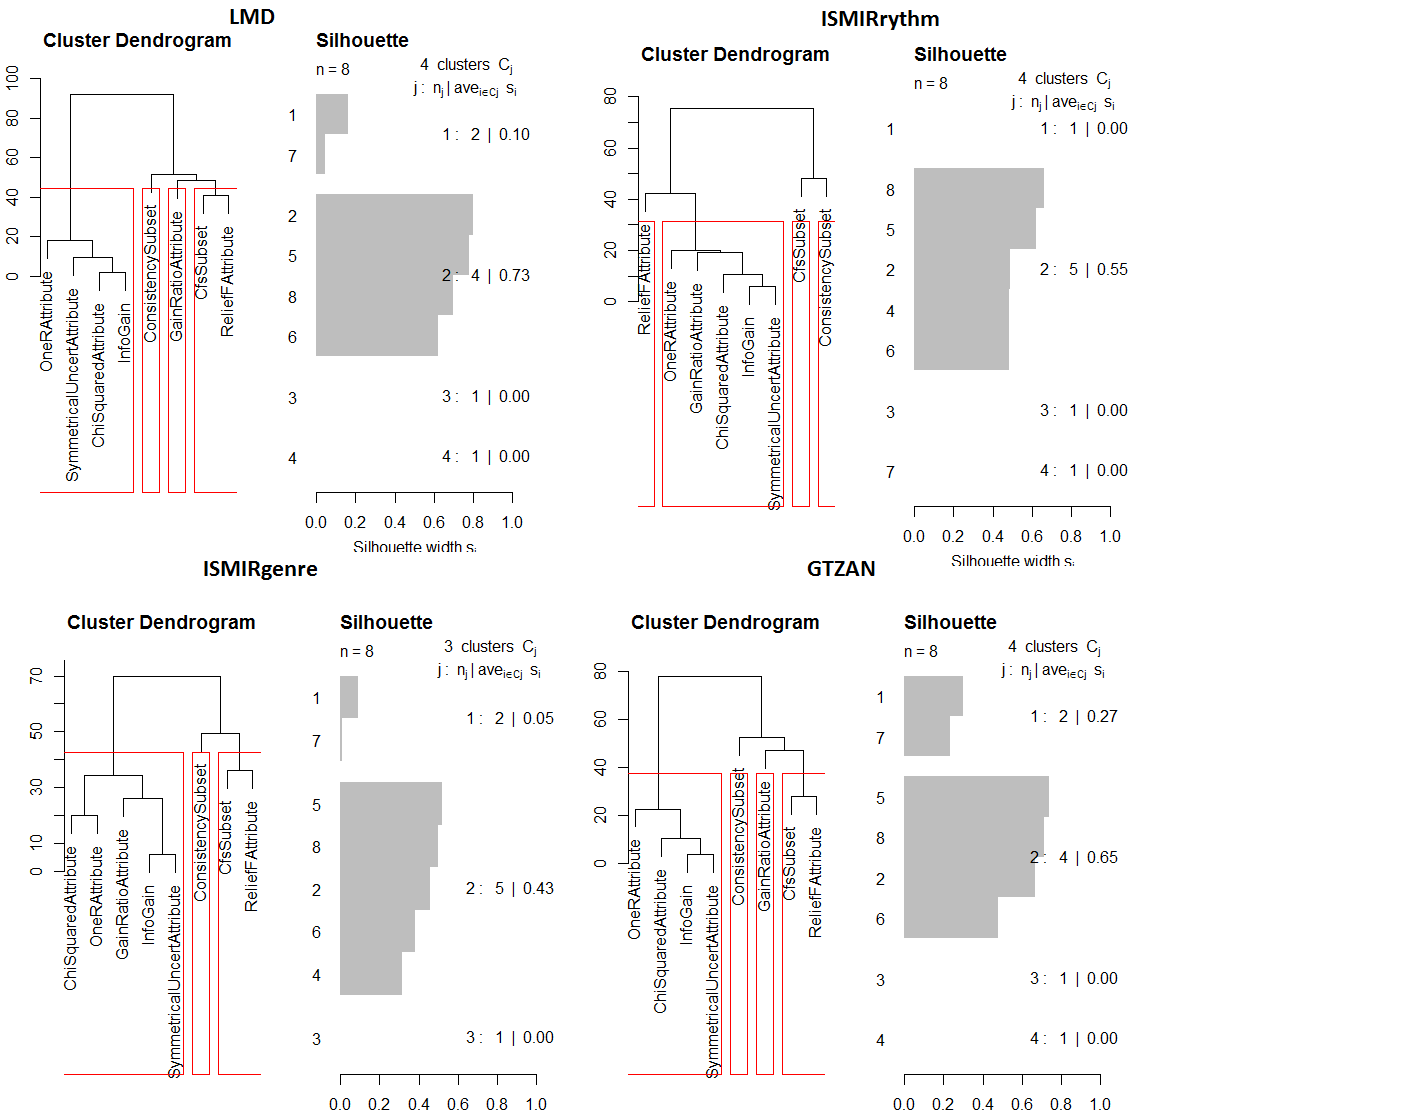
\includegraphics[scale=0.5]{fig/diagram_all.png}
\caption{Attribute selection methods clustering for four datasets
\label{fig:clustering}}
\end{center}
\end{figure}

\section{Comparison on Classifier}
\end{document}
